\documentclass[a4paper,11pt]{report}
\usepackage[spanish]{babel}
\usepackage[utf8]{inputenc}
\usepackage{graphicx, csquotes, longtable, array, booktabs, xparse, float, titlesec, enumitem, dingbat, soul, multicol, listings, wrapfig}
\usepackage[dvipsnames]{xcolor}
\usepackage[margin=2cm]{geometry}

% Añadir la bibliografía
\usepackage[backend=biber, style=numeric, sorting=ynt]{biblatex}
\addbibresource{memoria.bib}

% Cambia el color de los links
\usepackage{hyperref}
\hypersetup{hidelinks}

% Generamos un comando para saltar pagina con las secciones
\NewDocumentCommand{\cpsection}{s o m}{%
  \clearpage
  \IfBooleanTF{#1}
    {\section*{#3}}
    {%
      \IfNoValueTF{#2}
        {\section{#3}}
        {\section[#2]{#3}}%
    }%
}

\NewDocumentCommand{\cpsubsection}{s o m}{%
  \clearpage
  \IfBooleanTF{#1}
    {\subsection*{#3}}
    {%
      \IfNoValueTF{#2}
        {\subsection{#3}}
        {\subsection[#2]{#3}}%
    }%
}

% Elimina la palabra 'Capítulo' de los títulos de los capítulos
\titleformat{\chapter}[display]
  {\normalfont\bfseries}{}{0pt}{\Huge\thechapter.\space}

\titleformat{name=\chapter,numberless}[display]
  {\normalfont\bfseries}{}{0pt}{\Huge}

\titlespacing*{\chapter}{0pt}{-50pt}{20pt}

% Personalización del índice de listados
\renewcommand{\lstlistingname}{Código}  % Cambiar el nombre de 'Listing' a 'Código'
\renewcommand{\lstlistlistingname}{Índice de códigos}

% Añade numeración a los subsubsections y los añade al índice
\setcounter{secnumdepth}{4}
\setcounter{tocdepth}{4}

% Idioma predeterminado (Español)
\selectlanguage{spanish}

\begin{document}
  \begin{titlepage}
      \centering
      
\includegraphics[width=0.6\textwidth]{./.img/logo.jpg}\\
      \vspace{1cm}
      \Large Ingeniería Informática de Gestión y Sistemas de Información\\
      \vspace{3cm}
      \Huge Desarrollo Avanzado de Software\\
      \vspace{0.5cm}
      \huge \textbf{LibreBook}\\
      \vspace{7.5cm}
      \Large Estudiante:\\
      \vspace{0.2cm}
      \large Gabiña Barañano, Xabier\\
      \vspace{1cm}
      \vfill
      \today
  \end{titlepage}
  \tableofcontents
  \listoffigures
  \chapter{Introducción}
    \paragraph*{}{
      Al igual que en la primera entrega, LibreBook es una aplicación móvil para Android diseñada para los amantes de la lectura. Es una plataforma que permite a los usuarios crear una biblioteca personal digital donde pueden registrar, organizar y seguir su progreso en los libros que están leyendo o desean leer.
    }
    \paragraph*{}{
      La aplicación está desarrollada completamente en Java y sigue las mejores prácticas de desarrollo para Android, incluyendo el uso de Room para la persistencia de datos\cite{room_documentation}, arquitectura MVVM\cite{mvvm_pattern}, y componentes de la biblioteca de Material Design\cite{material_design} para ofrecer una interfaz moderna y funcional.\\
      El repositorio de la aplicación se encuentra en GitHub y está disponible para su descarga y uso bajo la licencia MIT.
    }
    \begin{center}
      %Link al repositorio
        \color{blue}\href{https://github.com/Xabierland/DAS-Proyecto}{Repositorio de la aplicación}
    \end{center}
    \paragraph*{}{
      Además en el repositorio, tambien esta disponible en GitHub el binario de la aplicación en formato apk para su descarga e instalación en dispositivos Android.
    }
    \begin{center}
      %Link al binario
        \color{blue}\href{https://github.com/Xabierland/DAS-Proyecto/releases}{Archivo APK de la aplicación}
    \end{center}
    \paragraph*{}{
      En la aplicación existen por defecto unicamente 10 libros.
      \begin{multicols}{2}
        \begin{enumerate}
          \item Crimen y Castigo
          \item Los Hermanos Karamazov
          \item El Idiota
          \item Memorias del Subsuelo
          \item El Jugador
          \item Los Demonios
          \item Humillados y Ofendidos
          \item El eterno marido
          \item Noches Blancas
          \item El doble
        \end{enumerate}
      \end{multicols}
      Todos de Dostoievski. Tenlo en cuenta a la hora de buscar los libros ya que no se pueden añadir libros directamente desde la aplicación.
    }
    \paragraph*{}{
      La aplicación cuenta con dos cuentas de usuario por defectos:
      \begin{itemize}
        \item \textbf{Administrador}
          \begin{itemize}
            \item Email: admin@xabierland.com
            \item Contraseña: admin
          \end{itemize}
        \item \textbf{Xabier}
          \begin{itemize}
            \item Email: xabierland@gmail.com
            \item Contraseña: 123456
          \end{itemize}
      \end{itemize}
      No obstante, se pueden crear nuevas cuentas de usuario mediante el registro en la aplicación.
    }  
  \chapter{Objetivos}
    \section{Elementos obligatorios}
      \begin{itemize}
        \item \textbf{Uso de una base de datos remota para el registro y la identificación de usuarios mediante registro.}
          \begin{itemize}
            \item Se ha migrado la base de datos de local a remota, manteniendo la misma estructura pero alojándola en un servidor externo.
            \item La definición de la base de datos se puede encontrar en \textbf{/sql/librebook\_db.sql}, con las mismas tablas que se utilizaban en la versión local (usuarios, libros, usuarios\_libros).
            \item Se ha desarrollado una API REST en PHP que sirve como intermediaria entre la aplicación Android y la base de datos MySQL (\textbf{/php/api.php}).
            \item Se han implementado nuevas clases en el paquete \textbf{com.xabierland.librebook.api} (ApiClient, ApiConfig, ApiParsers) para gestionar la comunicación con la API.
            \item Los repositorios (LibroRepository, UsuarioRepository, BibliotecaRepository) se han actualizado para realizar las operaciones CRUD a través de la API en lugar de hacerlo localmente.
          \end{itemize} 
        \item \textbf{Integrar los servicios Google Maps y Open Street Map y Geolocalización en una actividad.}
          \begin{itemize}
            \item Se ha implementado OpenStreetMap en la aplicación mediante la biblioteca OSMdroid.
            \item Se ha creado un nuevo fragmento (\textbf{MapFragment}) que muestra un mapa interactivo donde se visualizan las librerías cercanas a la ubicación del usuario.
            \item El fragmento gestiona los permisos de ubicación y utiliza el proveedor de ubicación de alta precisión de Google (FusedLocationProviderClient).
            \item Se ha implementado la clase utilitaria \textbf{BookstoreFinder} que utiliza la API de Overpass para buscar librerías y bibliotecas cercanas.
            \item Se muestran marcadores personalizados en el mapa para cada librería, con ventanas de información detallada al hacer clic (implementadas mediante \textbf{CustomInfoWindow}).
            \item El mapa se puede abrir desde la MainActivity a través de un card dedicado, mostrándose como un diálogo a pantalla completa.
          \end{itemize} 
        \item \textbf{Captar imágenes desde la cámara, guardarlas en el servidor y mostrarlas en la aplicación. Por ejemplo, una foto de perfil.}
          \begin{itemize}
            \item Se ha ampliado la funcionalidad de \textbf{ProfileActivity} para permitir a los usuarios tomar fotos con la cámara además de seleccionarlas desde la galería.
            \item Se han implementado los permisos necesarios para acceder a la cámara y al almacenamiento externo, con diálogos explicativos cuando se necesitan permisos.
            \item Se ha utilizado FileProvider para gestionar el acceso a archivos de imagen entre diferentes aplicaciones cámara y LibreBook.
            \item Se ha agregado la clase utilitaria \textbf{FileUtils} para procesar las imágenes, corregir su orientación y convertirlas a formato base64 para su almacenamiento.
            \item Las imágenes de perfil se transmiten al servidor codificadas en base64 a través de la API y se almacenan en la base de datos remota.
            \item Las imágenes se cargan correctamente en el menú de navegación y en las vistas de perfil propio y de otros usuarios.
          \end{itemize}
      \end{itemize}
    \section{Elementos opcionales}
      \begin{itemize}
        \item \textbf{Uso de algún Content Provider para añadir, modificar o eliminar datos.}
          \begin{itemize}
            \item Se ha implementado un Content Provider personalizado \textbf{LibreBooksProvider} que permite a otras aplicaciones acceder a los datos de libros de la biblioteca del usuario.
            \item El Content Provider expone dos tipos de URI: una para acceder a la lista de libros \textbf{books} y otra para obtener archivos de texto con información detallada de un libro específico \textbf{book\_files}.
            \item Se ha implementado la funcionalidad de compartir libros mediante este Content Provider en \textbf{BookDetailActivity} (botón de compartir en la barra de herramientas) y en \textbf{BookCardAdapter} (menú contextual al mantener pulsado un libro).
            \item La clase \textbf{ShareUtils} proporciona métodos para compartir información de libros como texto plano o como archivos de texto a través del Content Provider.
            \item El Content Provider permite compartir no solo la información básica del libro, sino también datos adicionales como el estado de lectura, calificación y notas personales.
          \end{itemize}
        \item \textbf{Implementación de un servicio en primer plano y gestión de mensajes broadcast durante el servicio}
          \begin{itemize}
            \item Se ha desarrollado un servicio en primer plano \textbf{ReadingTimerService} que permite al usuario registrar su tiempo de lectura incluso cuando la aplicación está en segundo plano.
            \item El servicio muestra una notificación persistente con el tiempo transcurrido y controles para detener el temporizador.
            \item Se ha implementado un sistema de comunicación bidireccional entre la actividad \textbf{ReadingTimerActivity} y el servicio mediante un mecanismo de binding y una interfaz de callback \textbf{TimerListener}.
            \item El servicio gestiona intents de tipo broadcast para responder a acciones como iniciar, detener y reiniciar el temporizador.
            \item Se ha configurado correctamente el servicio para ejecutarse en Android 12+ siguiendo las restricciones de ejecución en segundo plano y solicitando el tipo de servicio adecuado (FOREGROUND\_SERVICE\_DATA\_SYNC).
            \item La actividad se asegura de que el servicio siga funcionando incluso si el usuario cierra la aplicación, y puede reconectarse al servicio cuando se vuelve a abrir.
          \end{itemize}
        \item \textbf{Uso de mensajería FCM. Se debe incluir alguna forma de que se pueda probar de forma externa (por ejemplo, con un servicio web PHP adicional en el servidor de la asignatura).}
          \begin{itemize}
            \item Se ha implementado Firebase Cloud Messaging (FCM) para recibir notificaciones push en la aplicación.
            \item Se ha creado un servicio \textbf{LibreBookMessagingService} que extiende \textbf{FirebaseMessagingService} para gestionar los mensajes recibidos.
            \item La aplicación se suscribe automáticamente al tema "all\_devices" para recibir notificaciones generales.
            \item Se solicitan los permisos necesarios para mostrar notificaciones en Android 13+.
            \item Se ha implementado un panel de administración web accesible desde \href{http://ec2-51-44-167-78.eu-west-3.compute.amazonaws.com/xgabina001/WEB/admin_panel.php}{esta URL} que permite enviar notificaciones a todos los dispositivos suscritos.
            \item Las notificaciones pueden contener un título, un mensaje y abren la aplicación al ser pulsadas.
          \end{itemize}
        \item \textbf{Desarrollar un widget que tenga, al menos, un elemento que se actualice automáticamente de manera periódica.}
          \begin{itemize}
            \item Se ha implementado un widget de escritorio (\textbf{BookRecommendationWidgetProvider}) que muestra recomendaciones de libros aleatorios de la biblioteca del usuario.
            \item El widget se actualiza automáticamente cada 15 segundos mediante un AlarmManager para mostrar diferentes recomendaciones.
            \item El widget muestra la portada del libro, el título y el autor, y al pulsarlo, abre la actividad de detalle del libro correspondiente.
            \item Se ha implementado la clase utilitaria \textbf{WidgetImageLoader} para cargar imágenes desde URLs en el widget de forma asíncrona.
            \item El widget gestiona adecuadamente su ciclo de vida, incluyendo la cancelación de actualizaciones cuando se elimina y la programación de nuevas actualizaciones cuando se crea.
            \item Se han utilizado RemoteViews para diseñar la interfaz del widget, que se adapta a diferentes tamaños de pantalla.
          \end{itemize}
        \item \textbf{Uso de algún servicio o tarea programada mediante alarma (no valen las alarmas del widget).}
          \begin{itemize}
            \item Se ha implementado una actualización periódica de las recomendaciones de libros en la pantalla principal mediante un Handler y un Runnable en \textbf{MainActivity}.
            \item Cada 15 segundos, la aplicación actualiza la lista de libros recomendados con selecciones aleatorias de la biblioteca.
            \item La actualización periódica se inicia en \textbf{onResume()} y se detiene en \textbf{onPause()} para conservar recursos del sistema.
            \item La lógica de actualización está encapsulada en el método \textbf{loadRecommendedBooks()}, que obtiene los libros de forma asíncrona y actualiza la interfaz.
            \item Se utiliza un generador de números aleatorios con semilla basada en la hora actual para asegurar que las recomendaciones sean diferentes en cada actualización.
            \item La interfaz de usuario se actualiza de forma suave sin interrumpir la interacción del usuario con la aplicación.
          \end{itemize}
      \end{itemize}
  \chapter{Descripción de la aplicación}
    \section{Clases}
      \begin{figure}[H]
        \centering
        \href{https://raw.githubusercontent.com/Xabierland/DAS-Proyecto/refs/heads/main/Documentation/Memoria2/.img/diagrama-clases.svg}{%
          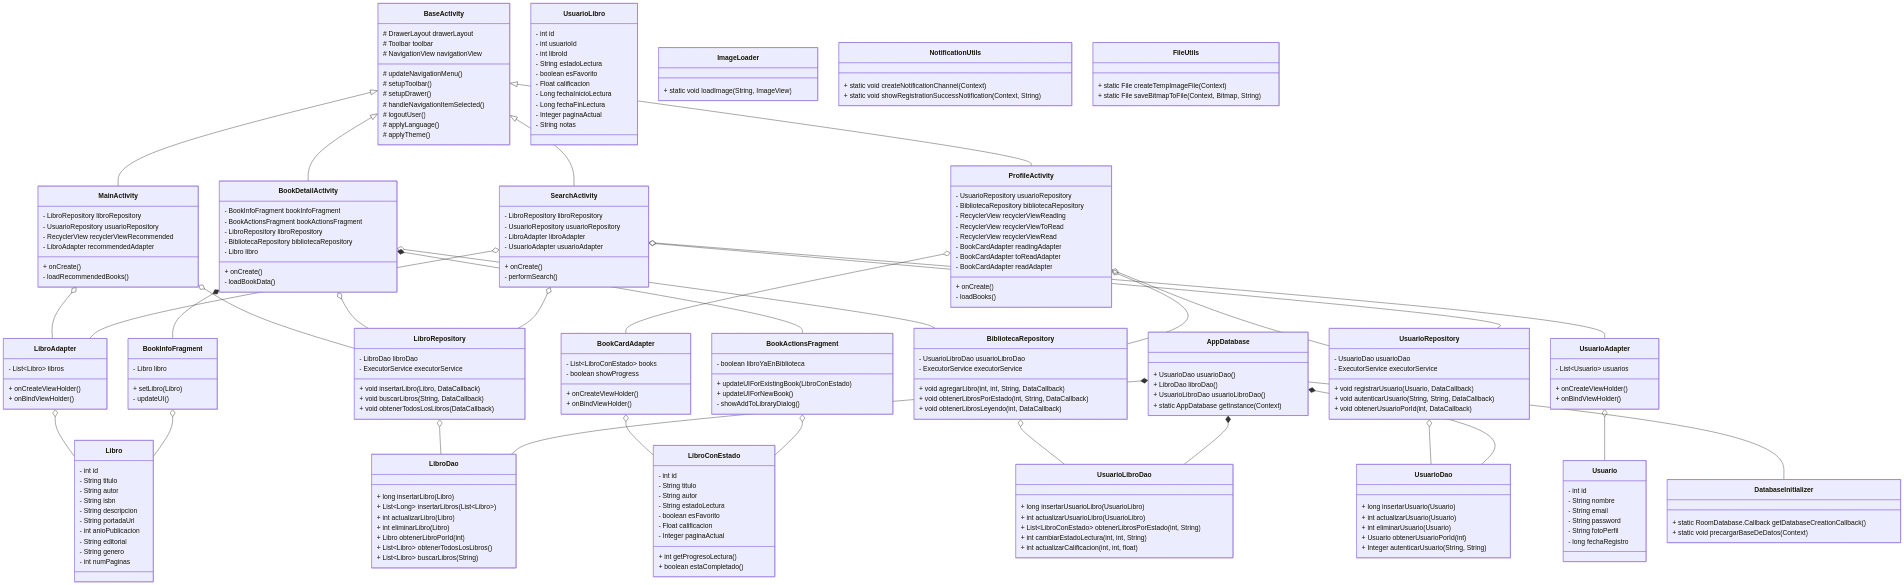
\includegraphics[width=0.9\textwidth]{.img/diagrama-clases.png}
        }
        \caption{Diagrama de clases de la aplicación LibreBook}
        \label{fig:diagrama-clases}
      \end{figure}
      Como se muestra en la Figura~\ref{fig:diagrama-clases}, la ha aumentado el número de clases respecto a la entrega anterior pero manteniendo las capas con una clara separación de responsabilidades\cite{android_architecture}:
      En este apartado me voy a limitar a describir los cambios realizados en la aplicación respecto a la entrega anterior.
      \subsection{Activities}
        \begin{itemize}
          \item \textbf{Modificaciones en ProfileActivity:} Se ha ampliado para permitir la captura de imágenes mediante la cámara o su selección desde la galería, ajustarlas y guardarlas como fotos de perfil.
          \item \textbf{ReadingTimerActivity:} Interfaz de usuario para controlar el temporizador de lectura, permitiendo iniciar, pausar y reiniciar el tiempo de lectura.
        \end{itemize}
      \subsection{Fragments}
        \begin{itemize}
          \item \textbf{MapFragment:} Fragment que muestra un mapa interactivo con las librerías cercanas a la ubicación del usuario utilizando OpenStreetMap.
        \end{itemize}
      \subsection{Services}
        \begin{itemize}
          \item \textbf{ReadingTimerService:} Implementa un servicio en primer plano que mantiene un temporizador de lectura activo incluso cuando la aplicación está en segundo plano. Muestra una notificación persistente que se actualiza con el tiempo transcurrido.
          \item \textbf{LibreBookMessagingService:} Extiende FirebaseMessagingService para recibir y procesar mensajes push. Gestiona tanto mensajes de notificación como mensajes de datos.
        \end{itemize}
      \subsection{API}
        \begin{itemize}
          \item \textbf{ApiClient:} Proporciona métodos genéricos para realizar peticiones HTTP (GET, POST, PUT, DELETE) a nuestra API REST. Gestiona la comunicación asíncrona y el manejo de errores.
          \item \textbf{ApiConfig:} Contiene la configuración básica como la URL base de la API.
          \item \textbf{ApiParsers:} Conjunto de parseadores que convierten las respuestas JSON en objetos del dominio de la aplicación (Libro, Usuario, LibroConEstado, etc.).
        \end{itemize}
      \subsection{Provider}
        \begin{itemize}
          \item \textbf{LibreBooksProvider:} Content Provider que permite a otras aplicaciones acceder a la información de libros de LibreBook.
        \end{itemize}
      \subsection{Widget}
        \begin{itemize}
          \item \textbf{BookRecommendationWidgetProvider:} Implementa un widget de escritorio que muestra recomendaciones de libros y se actualiza periódicamente.
        \end{itemize}
      \subsection{Repositorios}
        \begin{itemize}
          \item \textbf{Modificaciones en LibroRepository:} Actualizado para interactuar con la API REST en lugar de la base de datos local. Proporciona métodos para obtener, añadir, modificar y eliminar libros.
          \item \textbf{Modificaciones en UsuarioRepository:} Actualizado para interactuar con la API REST en lugar de la base de datos local.. Proporciona métodos para gestionar usuarios y autenticación.
          \item \textbf{Modificaciones en BibliotecaRepository:} Actualizado para interactuar con la API REST en lugar de la base de datos local.. Proporciona métodos para gestionar la biblioteca del usuario.
        \end{itemize}
      \subsection{Utils}
        \begin{itemize}
          \item \textbf{BookstoreFinder:} Clase utilitaria que utiliza la API de Overpass para buscar librerías y bibliotecas cercanas a una ubicación dada.
          \item \textbf{CustomInfoWindow:} Componente personalizado para mostrar información detallada sobre una librería al seleccionar su marcador en el mapa.
          \item \textbf{ShareUtils:} Proporciona métodos para compartir información de libros como texto plano o como archivos de texto.
          \item \textbf{WidgetImageLoader:} Clase utilitaria para cargar imágenes de portadas de libros en el widget.
          \item \textbf{FileUtils:} Proporciona métodos para gestionar archivos, convertir entre diferentes formatos de imagen y corregir orientación de imágenes capturadas.
        \end{itemize}
    \cpsection{Base de datos}
      \begin{figure}[H]
        \centering
        \href{https://raw.githubusercontent.com/Xabierland/DAS-Proyecto/refs/heads/main/Documentation/Memoria2/.img/diagrama-bd.svg}{%
          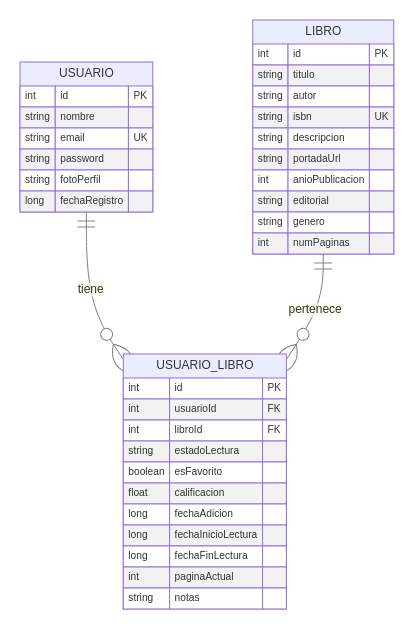
\includegraphics[width=0.4\textwidth]{.img/diagrama-bd.png}
        }
        \caption{Diagrama de la base de datos de la aplicación LibreBook}
        \label{fig:diagrama-bd}
      \end{figure}
      La base de datos no ha sufrido cambios respecto en su estructura respecto a la entrega anterior.
  \chapter{Manual de usuario}
    \section{Base de datos remota con API}
      Ahora la base de datos de la aplicación está alojada en un servidor remoto y se accede a ella a través de una API REST. Esto permite que los datos sean accesibles desde cualquier dispositivo con conexión a Internet y facilita la sincronización entre diferentes instancias de la aplicación.
      Es posible ver parte de la información de la base de datos desde los seguientes endpoints:
      \begin{itemize}
        \item \href{http://ec2-51-44-167-78.eu-west-3.compute.amazonaws.com/xgabina001/WEB/api.php/usuarios}{http://ec2-51-44-167-78.eu-west-3.compute.amazonaws.com/xgabina001/WEB/api.php/usuarios} \\Usuarios
        \item \href{http://ec2-51-44-167-78.eu-west-3.compute.amazonaws.com/xgabina001/WEB/api.php/libros}{http://ec2-51-44-167-78.eu-west-3.compute.amazonaws.com/xgabina001/WEB/api.php/libros} \\Libros
        \item \href{http://ec2-51-44-167-78.eu-west-3.compute.amazonaws.com/xgabina001/WEB/api.php/biblioteca/2}{http://ec2-51-44-167-78.eu-west-3.compute.amazonaws.com/xgabina001/WEB/api.php/biblioteca/2} \\Biblioteca del usuario 2
        \item \href{http://ec2-51-44-167-78.eu-west-3.compute.amazonaws.com/xgabina001/WEB/api.php/biblioteca/1?estado=leyendo}{http://ec2-51-44-167-78.eu-west-3.compute.amazonaws.com/xgabina001/WEB/api.php/biblioteca/2?estado=leyendo} \\Libros que esta leyendo el usuario 2
      \end{itemize}
      De esta forma conseguimos que la aplicación sea más escalable y flexible, permitiendo futuras mejoras y nuevas funcionalidades sin necesidad de realizar cambios significativos en la arquitectura de la aplicación.
    \cpsection{Encontrar librerías}
      Para que los usuarios puedan encontrar librerías cercanas a su ubicación, se ha implementado un mapa interactivo.
      \begin{figure}[H]
        \centering
        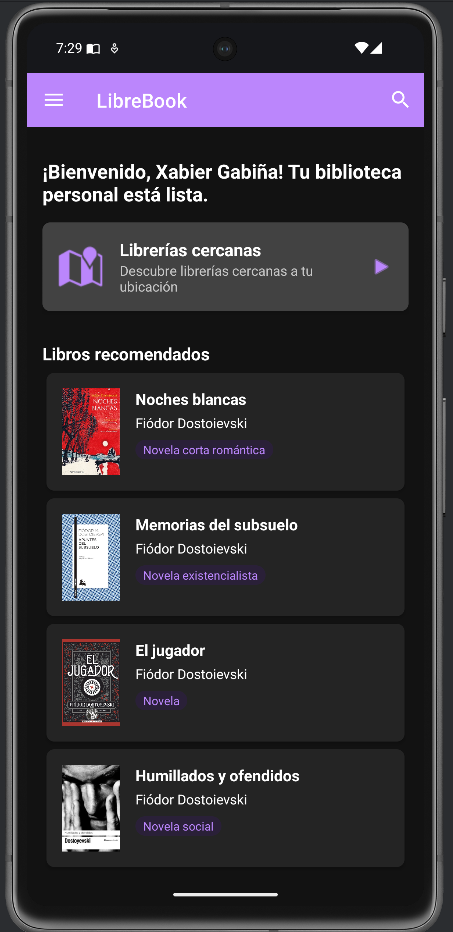
\includegraphics[width=0.25\textwidth]{.img/mapa_boton.png}
        \hspace{2cm}
        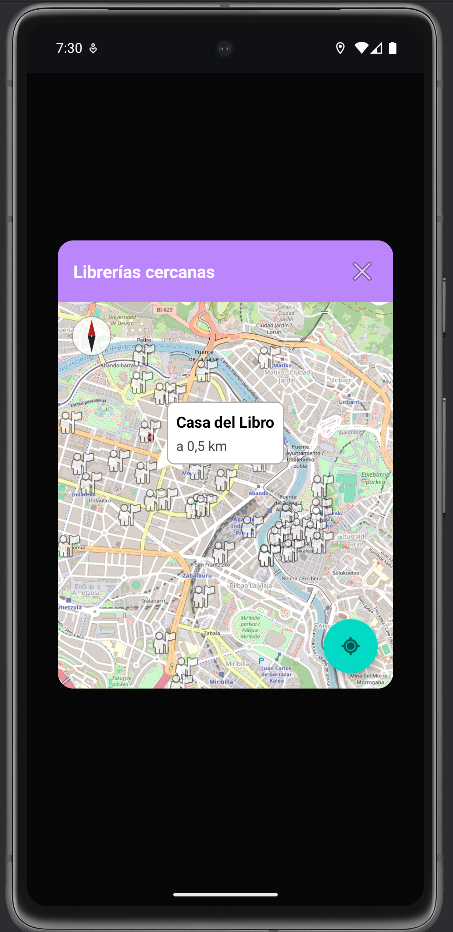
\includegraphics[width=0.25\textwidth]{.img/mapa_fragment.png}
        \caption{Encontrar librerías}
        \label{fig:mapa}
      \end{figure}
      En la pantalla principal de la aplicación, se encuentra un boton de Librerias cercanas que al pulsarlo abre un mapa interactivo con las librerías cercanas a la ubicación del usuario. 
      El mapa se muestra a pantalla completa, permitiendo al usuario desplazarse, hacer zoom y interactuar con los iconos para ver las librerias y la distancia a la que se encuentran.
    \cpsection{Foto de perfil}
      Aunque en la entrega anterior era posible elegir una foto de la galería ahora tambien es posible usar la camara del movil para subir una foto de perfil a la aplicación conservando ademas la opcion de la galeria y sincronizandola con la base de datos.
      \begin{figure}[H]
        \centering
        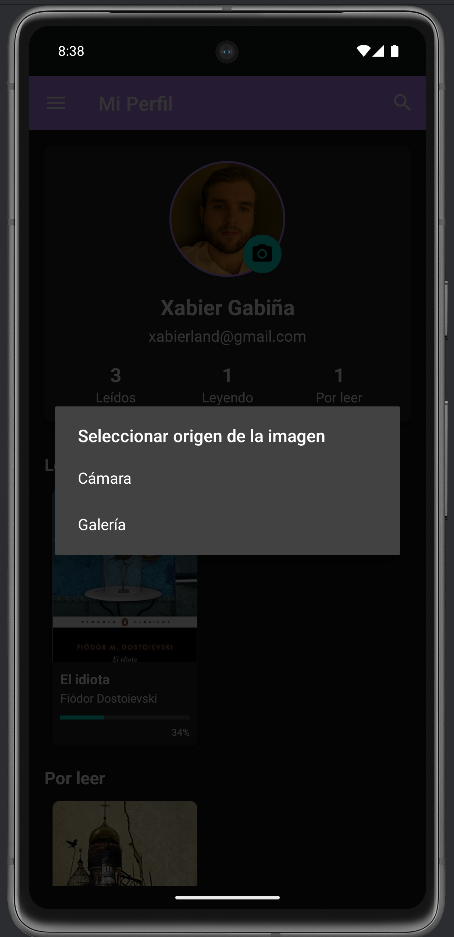
\includegraphics[width=0.25\textwidth]{.img/foto_perfil_1.png}
        \hspace{1cm}
        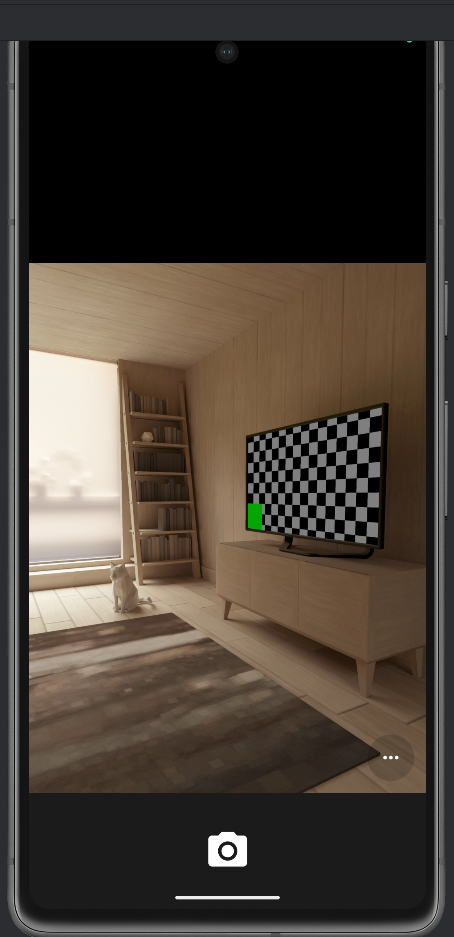
\includegraphics[width=0.25\textwidth]{.img/foto_perfil_2.png}
        \hspace{1cm}
        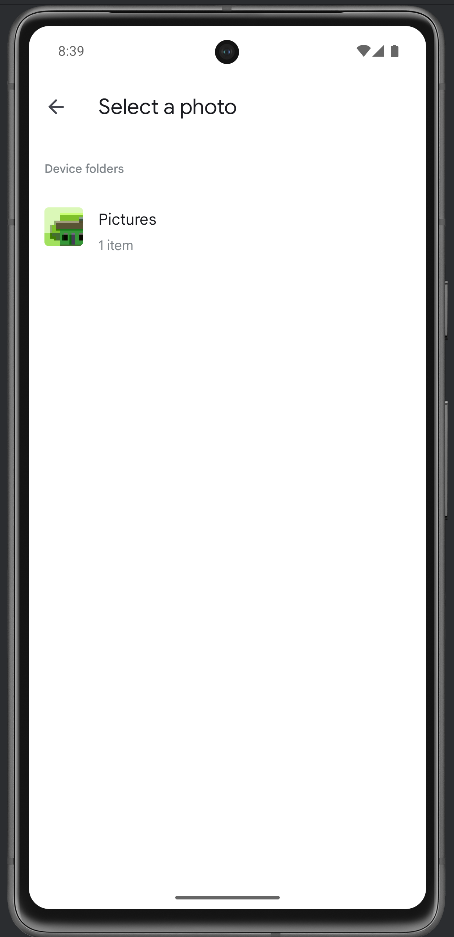
\includegraphics[width=0.25\textwidth]{.img/foto_perfil_3.png}
        \caption{Foto de perfil}
        \label{fig:perfil}
      \end{figure}
      Para elegirla entra desde el menu desplegable de la aplicacion en el perfil del usuario y dale click al icono de la camara al lado de la foto de perfil.
      Al pulsar el icono de la cámara, se abre un diálogo que permite al usuario elegir entre tomar una foto con la cámara o seleccionar una imagen de la galería.
    \cpsection{Compartir libros}
      La aplicación permite compartir libros con otros usuarios mediante dos métodos:
      \begin{figure}[H]
        \centering
        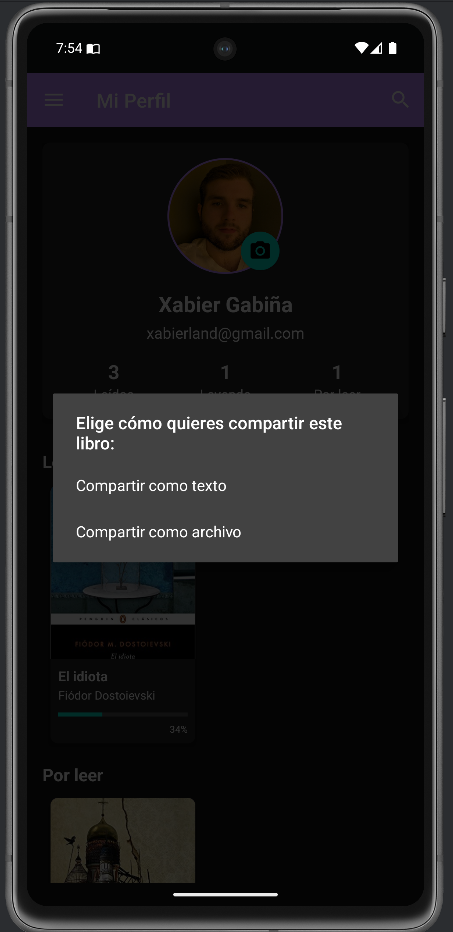
\includegraphics[width=0.25\textwidth]{.img/compartir_perfil.png}
        \caption{Compartir libros desde el perfil}
        \label{fig:compartir-perfil}
      \end{figure}
      El primero como se ven en la Figura~\ref{fig:compartir-perfil} es desde el perfil de usuario, donde al mantener pulsado un libro se abre un menú contextual que permite compartir el libro seleccionado.
      \begin{figure}[H]
        \centering
        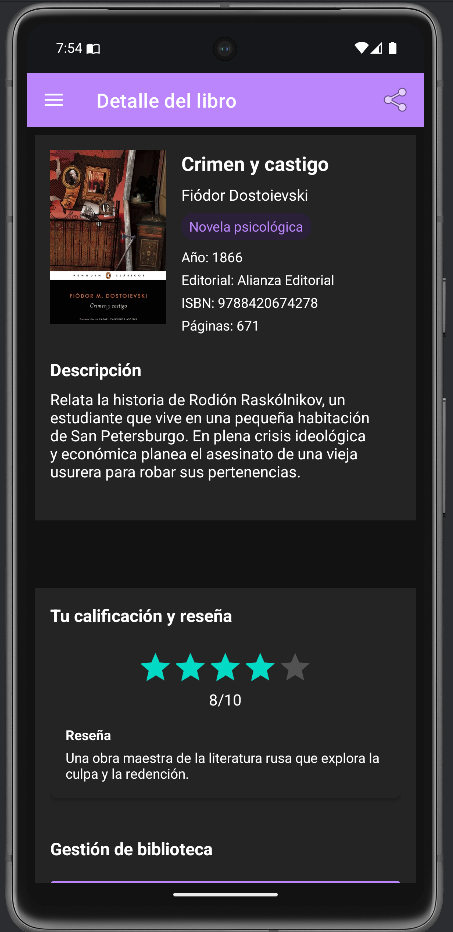
\includegraphics[width=0.25\textwidth]{.img/compartir_libro_1.png}
        \hspace{2cm}
        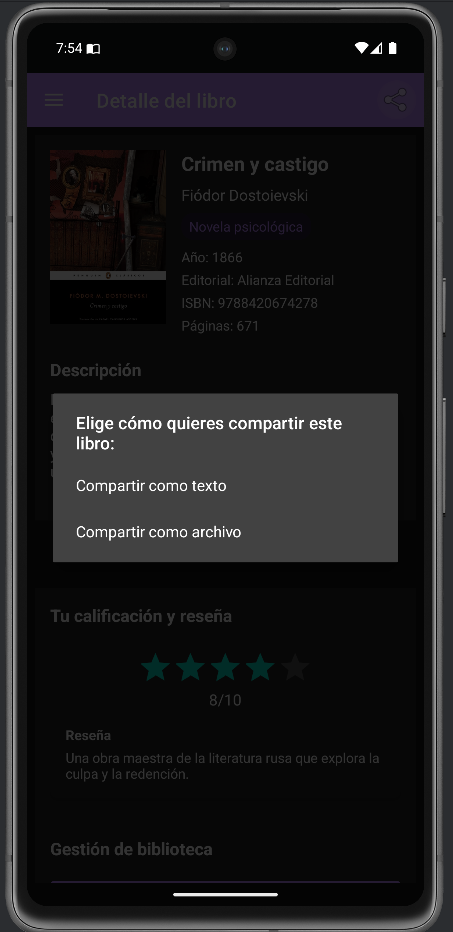
\includegraphics[width=0.25\textwidth]{.img/compartir_libro_2.png}
        \caption{Compartir libros desde la vista de libro}
        \label{fig:compartir-libro}
      \end{figure}
      La segunda opción es desde la vista de libro, donde en la parte superior derecha de la pantalla se encuentra un icono de compartir. Al pulsar este icono, se abre un menú que permite al usuario elegir entre compartir el libro como texto plano o como archivo de texto.
    \cpsection{Temporizador de lectura}
      La aplicación cuenta con un temporizador de lectura que permite a los usuarios registrar el tiempo que pasan leyendo.
      \begin{figure}[H]
        \centering
        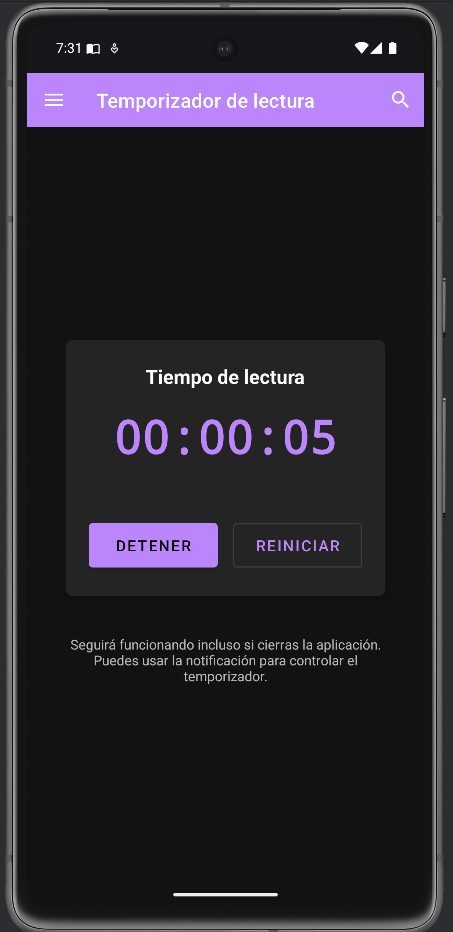
\includegraphics[width=0.25\textwidth]{.img/temporizador.png}
        \hspace{2cm}
        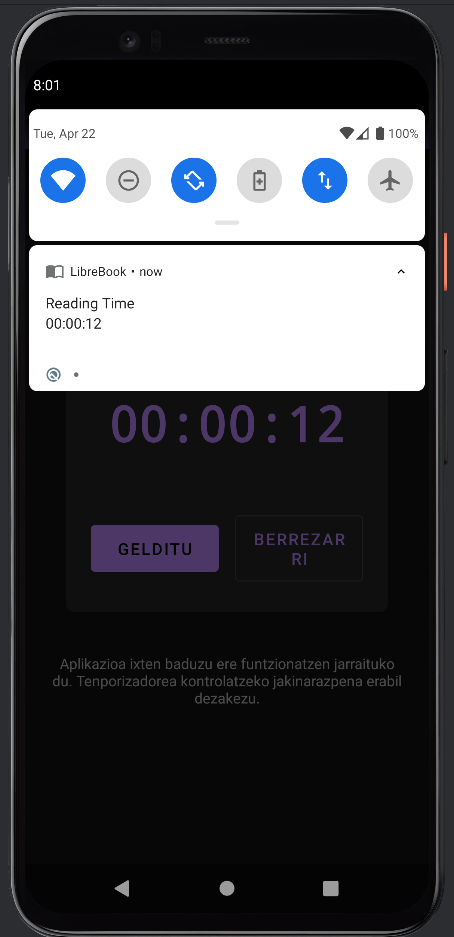
\includegraphics[width=0.25\textwidth]{.img/temporizador_2.png}
        \caption{Temporizador de lectura}
        \label{fig:temporizador}
      \end{figure}
      El temporizador funciona incluso con la aplicacion cerrada, mostrando una notificación persistente que se actualiza cada segundo con el tiempo transcurrido.
      El usuario puede iniciar, pausar y reiniciar el temporizador desde la interfaz de la aplicación. Al abrir la aplicación, el temporizador se reanuda automáticamente y se muestra el tiempo total acumulado.
    \cpsection{Mensajeria FCM}
      La aplicación utiliza Firebase Cloud Messaging (FCM) para recibir notificaciones push. Los usuarios pueden enviar mensajes a todos los dispositivos a través de un \textcolor{blue}{\href{http://ec2-51-44-167-78.eu-west-3.compute.amazonaws.com/xgabina001/WEB/admin_panel.php}{panel de administración web}}.
      \begin{figure}[H]
        \centering
        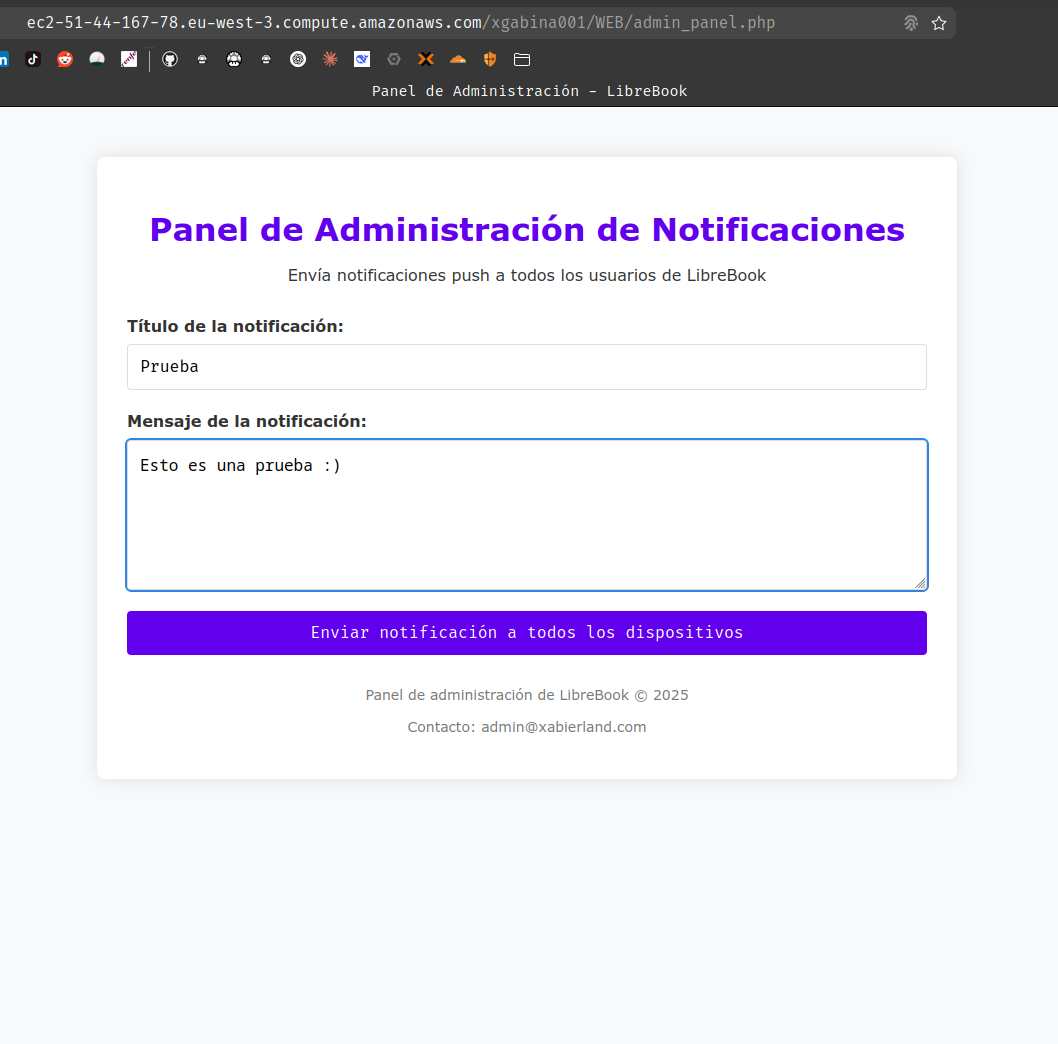
\includegraphics[width=0.4\textwidth]{.img/mensaje_no_enviado.png}
        \hspace{2cm}
        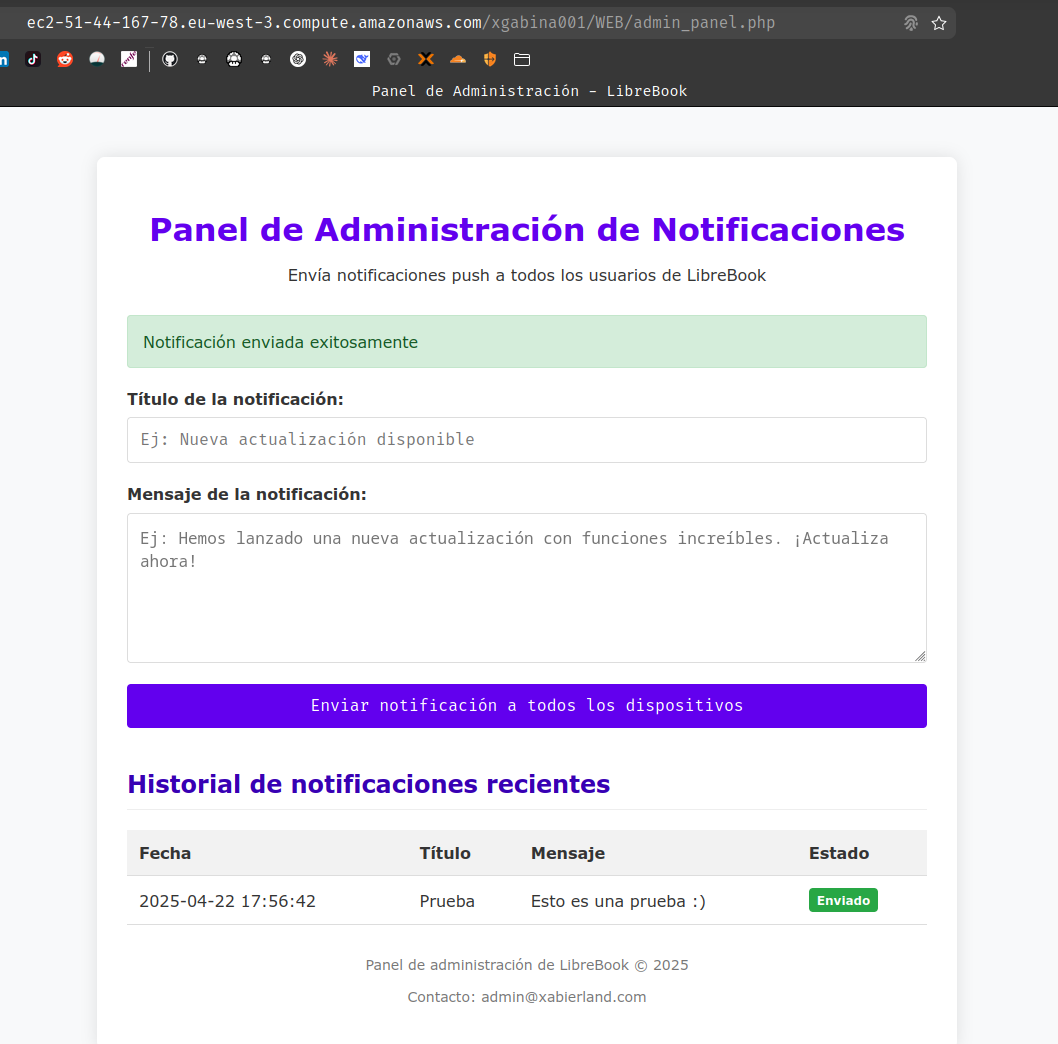
\includegraphics[width=0.4\textwidth]{.img/mensaje_enviado.png}
        \caption{Interfaz para enviar mensaje mediante FCM}
        \label{fig:mensaje}
      \end{figure}
      \begin{figure}[H]
        \centering
        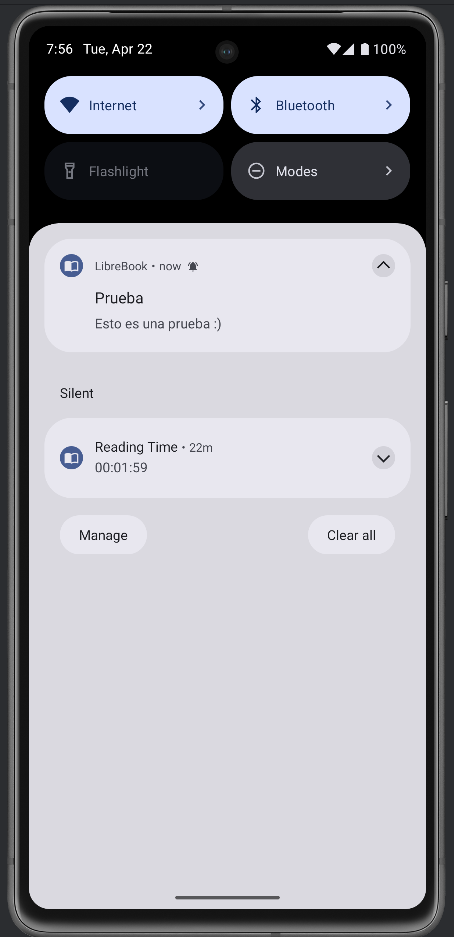
\includegraphics[width=0.25\textwidth]{.img/mensaje_notificacion.png}
        \caption{Notificación recibida}
        \label{fig:mensaje-notificacion}
      \end{figure}
      De esta forma los usuarios pueden recibir mensajes importantes, actualizaciones o recordatorios directamente en su dispositivo móvil.
    \cpsection{Widget}
      Junto con la aplicacion se añade un widget para colocar en el escritorio del movil.
      \begin{figure}[H]
        \centering
        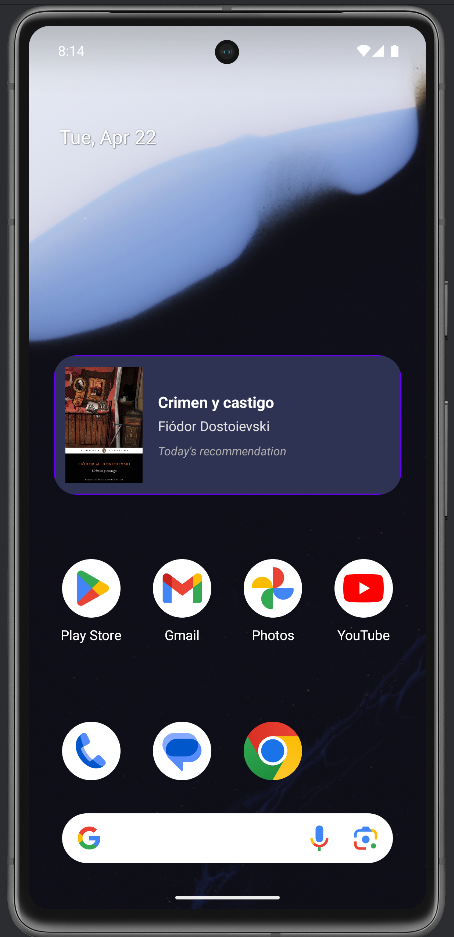
\includegraphics[width=0.25\textwidth]{.img/widget.png}
        \hspace{2cm}
        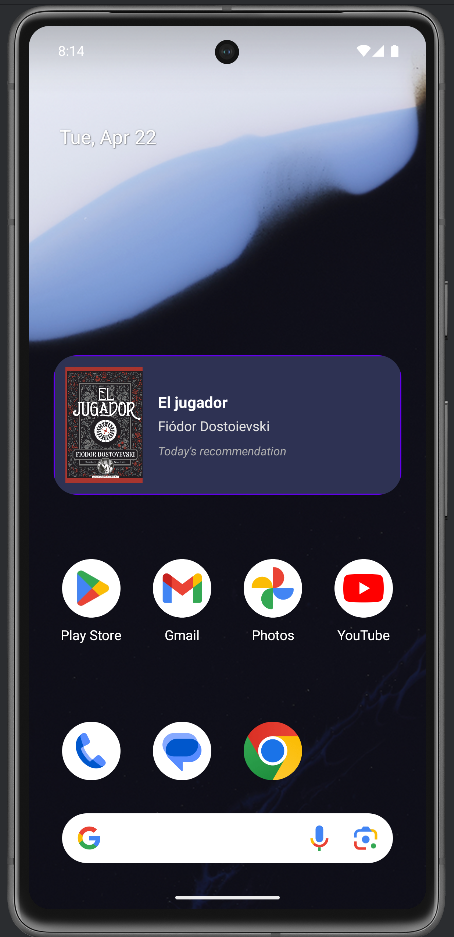
\includegraphics[width=0.25\textwidth]{.img/widget_2.png}
        \caption{Widget de la aplicación}
        \label{fig:widget}
      \end{figure}
      El widget muestra recomendaciones de libros aleatorios de la biblioteca del usuario. Se actualiza automáticamente cada 15 segundos para mostrar diferentes recomendaciones.
      Al pulsar el widget, se abre la actividad de detalle del libro correspondiente, permitiendo al usuario acceder rápidamente a la información del libro recomendado.
    \cpsection{Actualizar libros recomendados}
      Ahora la pagina principal de la aplicacion se actualiza cada 15 segundos para mostrar libros recomendados aleatorios de la biblioteca del usuario.
      \begin{figure}[H]
        \centering
        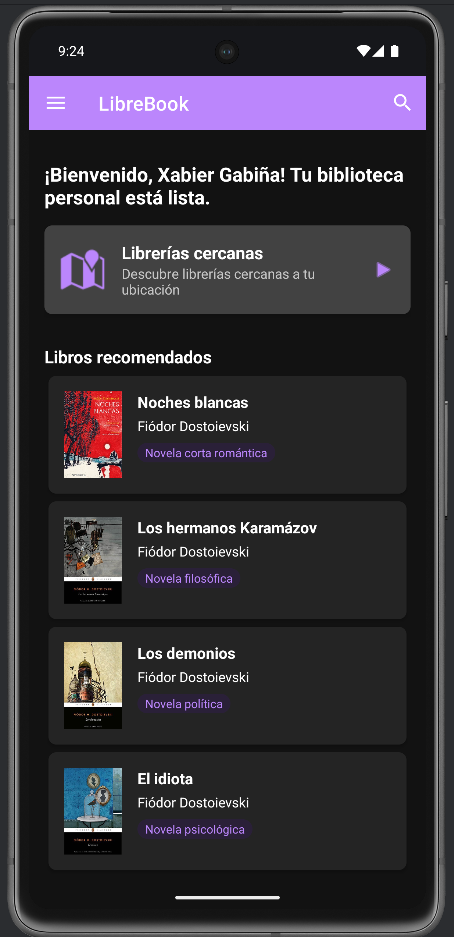
\includegraphics[width=0.25\textwidth]{.img/libros_recomendados_1.png}
        \hspace{2cm}
        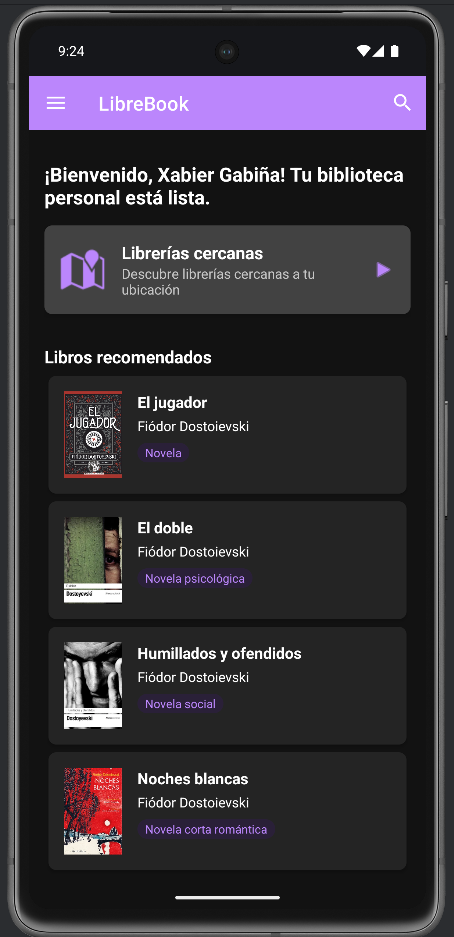
\includegraphics[width=0.25\textwidth]{.img/libros_recomendados_2.png}
        \caption{Libros recomendados}
        \label{fig:libros-recomendados}
      \end{figure}
  \chapter{Dificultades}
    Durante el desarrollo de esta segunda fase de LibreBook, me enfrenté a varios desafíos técnicos que tuve que resolver para implementar las nuevas funcionalidades.
    \section{Migración a base de datos remota}
      Cambiar de una base de datos local a una remota resultó más complicado de lo esperado:
      \begin{itemize}
        \item Al haber usado Room en la fase anterior, no tenía las sentencias SQL explícitas para crear la estructura en el servidor, por lo que tuve que reconstruirlas manualmente analizando las entidades y relaciones.
        \item Fue necesario desarrollar una API REST completa en PHP que sirviera como intermediaria entre la aplicación Android y la base de datos MySQL del servidor.
        \item Todos los repositorios que antes funcionaban directamente con Room debían ahora comunicarse a través de la API, lo que implicó reescribir la lógica de acceso a datos.
        \item Tuve que implementar un sistema de parsing JSON en ambas direcciones: para enviar datos a la API (serialización) y para recibir e interpretar sus respuestas (deserialización).
        \item La gestión de errores se volvió más compleja, ya que además de los errores de la base de datos ahora debía manejar posibles fallos de red, timeouts o respuestas inesperadas del servidor.
      \end{itemize}
      La solución fue crear una capa de abstracción con clases específicas (ApiClient, ApiConfig, ApiParsers) que encapsularan toda la lógica de comunicación con el servidor y proporcionaran una interfaz similar a la que usaban los repositorios con Room, minimizando así los cambios en el resto de la aplicación.
    \section{Implementación del servicio de temporizador}
      El desarrollo del temporizador de lectura presentó desafíos particulares:
      \begin{itemize}
        \item Mi idea inicial fue usar WorkManager con tareas periódicas para actualizar el temporizador, pero descubrí que Android limita la frecuencia mínima a 15 minutos, lo que resultaba inútil para un cronómetro que necesita actualizarse cada segundo.
        \item Opté entonces por un servicio en primer plano (ForegroundService), pero tuve que lidiar con las restricciones que Android ha ido añadiendo en versiones recientes para limitar las aplicaciones que se ejecutan en segundo plano.
        \item La gestión del ciclo de vida del servicio fue complicada: necesitaba que el temporizador siguiera funcionando aunque el usuario cerrara la aplicación, pero también que la actividad pudiera reconectarse al servicio al volver a abrirla.
        \item Implementar la comunicación bidireccional entre la actividad y el servicio requirió configurar correctamente el mecanismo de binding y diseñar una interfaz de callback que permitiera actualizar la UI en tiempo real.
        \item La notificación persistente debía actualizarse cada segundo mostrando el tiempo transcurrido y ofrecer controles para detener el temporizador sin necesidad de abrir la aplicación.
      \end{itemize}
      Tras varios intentos, conseguí una solución funcional combinando un Handler para las actualizaciones por segundo, un servicio en primer plano que se mantiene activo incluso cuando la aplicación no está en uso, y un sistema de binding que permite a la actividad comunicarse con el servicio cuando está visible.
      \chapter{Conclusiones}
        Esta segunda fase del proyecto LibreBook ha supuesto un salto importante en la madurez de la aplicación, transformándola de una simple herramienta de gestión de biblioteca personal a una plataforma más completa con funcionalidades sociales, interactivas y en tiempo real. Gracias a la migración a una base de datos remota, la integración de mapas, el temporizador de lectura, el sistema de compartición mediante Content Provider, el widget de recomendaciones y las notificaciones push, la aplicación ahora ofrece una experiencia mucho más rica para los amantes de la lectura.\\
        
        Aunque el desarrollo de esta fase ha sido más complejo que la anterior, las dificultades superadas han resultado en una aplicación más robusta y completa. La experiencia de implementar estas funcionalidades avanzadas me ha permitido profundizar en temas como arquitecturas cliente-servidor, servicios en primer plano, geolocalización y mensajería en la nube, ampliando significativamente mis conocimientos en desarrollo Android. LibreBook ha evolucionado notablemente y, aunque hay aspectos que podrían mejorarse en el futuro (como la sincronización diferencial de datos o asociar el temporizador a libros específicos), estoy satisfecho con los resultados obtenidos y entusiasmado por las posibilidades de expansión que tiene la aplicación.
  \printbibliography[title=Bibliografía]
\end{document}